\providecommand{\main}{..}
\documentclass[\main/main.tex]{subfiles}

\begin{document}
\graphicspath{{img/}{position_estimation/img/}}
\chapter{Position estimation}

In this chapter, a position estimation technique is introduced. The ultimate aim of this technique is to be simple enough to run on a microcontroller while providing reasonable accuracy. Section \ref{sec:distance_measurement_using_time_of_flight} discusses about a technique used for distance measurement. A solution for solving location from distance to known points is proposed in chapter \ref{sec:localization_using_multilateration}.

\section{Distance measurement using time-of-flight}
\label{sec:distance_measurement_using_time_of_flight}

\subsection{RSSI vs Time of Flight Distance Estimation}
Generally, there are two ways to measure distances between two devices. The first is based on RSSI, or Received Signal Strength Indication. We know that the signal strength drops with increasing distance from the transmitter in a deterministic fashion that is based on theoretic formulas. With this assumption, we can estimate the distance between a receiver and transmitter. However, this approach has several disadvantages. Since the environment and thus the radio channel changes constantly, then so does the RSSI parameter, which in turn brings inaccuracy to the system. The RSSI parameter can be also degraded by multipath propagation and other phenomenons that are quite common for the radio channel. The results and the overall accuracy can be increased by a process called fingerprinting, however due to rapidly changing radio environments, this process would need to be done frequently to improve the ranging results. Traditional technologies like Wi-Fi, Bluetooth, Bluetooth Low Energy and Active RFID are based on this distance estimation process.

Another option is to use the signal’s Time of Flight rather than RSSI. This yields much more accurate results in Line of Sight environments and can lead up to a centimeter level accuracy depending on the frequency and nature of the signal. This is an approach that is used by the Ultra Wideband technology. By combining the Time of Flight measurements from several devices, we can obtain an accurate position with precision of up to several centimeters. The nature of UWB signals makes it an ideal candidate for utilizing the Time of Flight distance estimation process. The performance might be degraded for example by obscuring the Line of Sight between UWB devices, however the overall accuracy is still superior in comparison to RSSI.

Time of Flight (ToF) is a method for measuring the distance between two radio transceivers by multiplying the Time of Flight of the signal by the speed of light. From this basic principle, UWB technology can be implemented in different ways based on the target applications needs: Two Way Ranging (TWR), Time Difference of Arrival (TDoA), or Phase Difference of Arrival (PDoA).

\subsection{Time Difference of Arrival (TDoA)}
The TDoA method is very similar to GPS. Multiple reference points, called anchors, are deployed in a venue and are time synchronized. The mobile devices will beacon, and when an anchor receives the beacon signal it will timestamp it. The timestamps from multiple anchors are then sent back to a central location engine which will run multilateration algorithms based on Time Difference of Arrival of the beacons signals to compute the X, Y, Z of the mobile devices.

\begin{figure}[H]
    \centering
    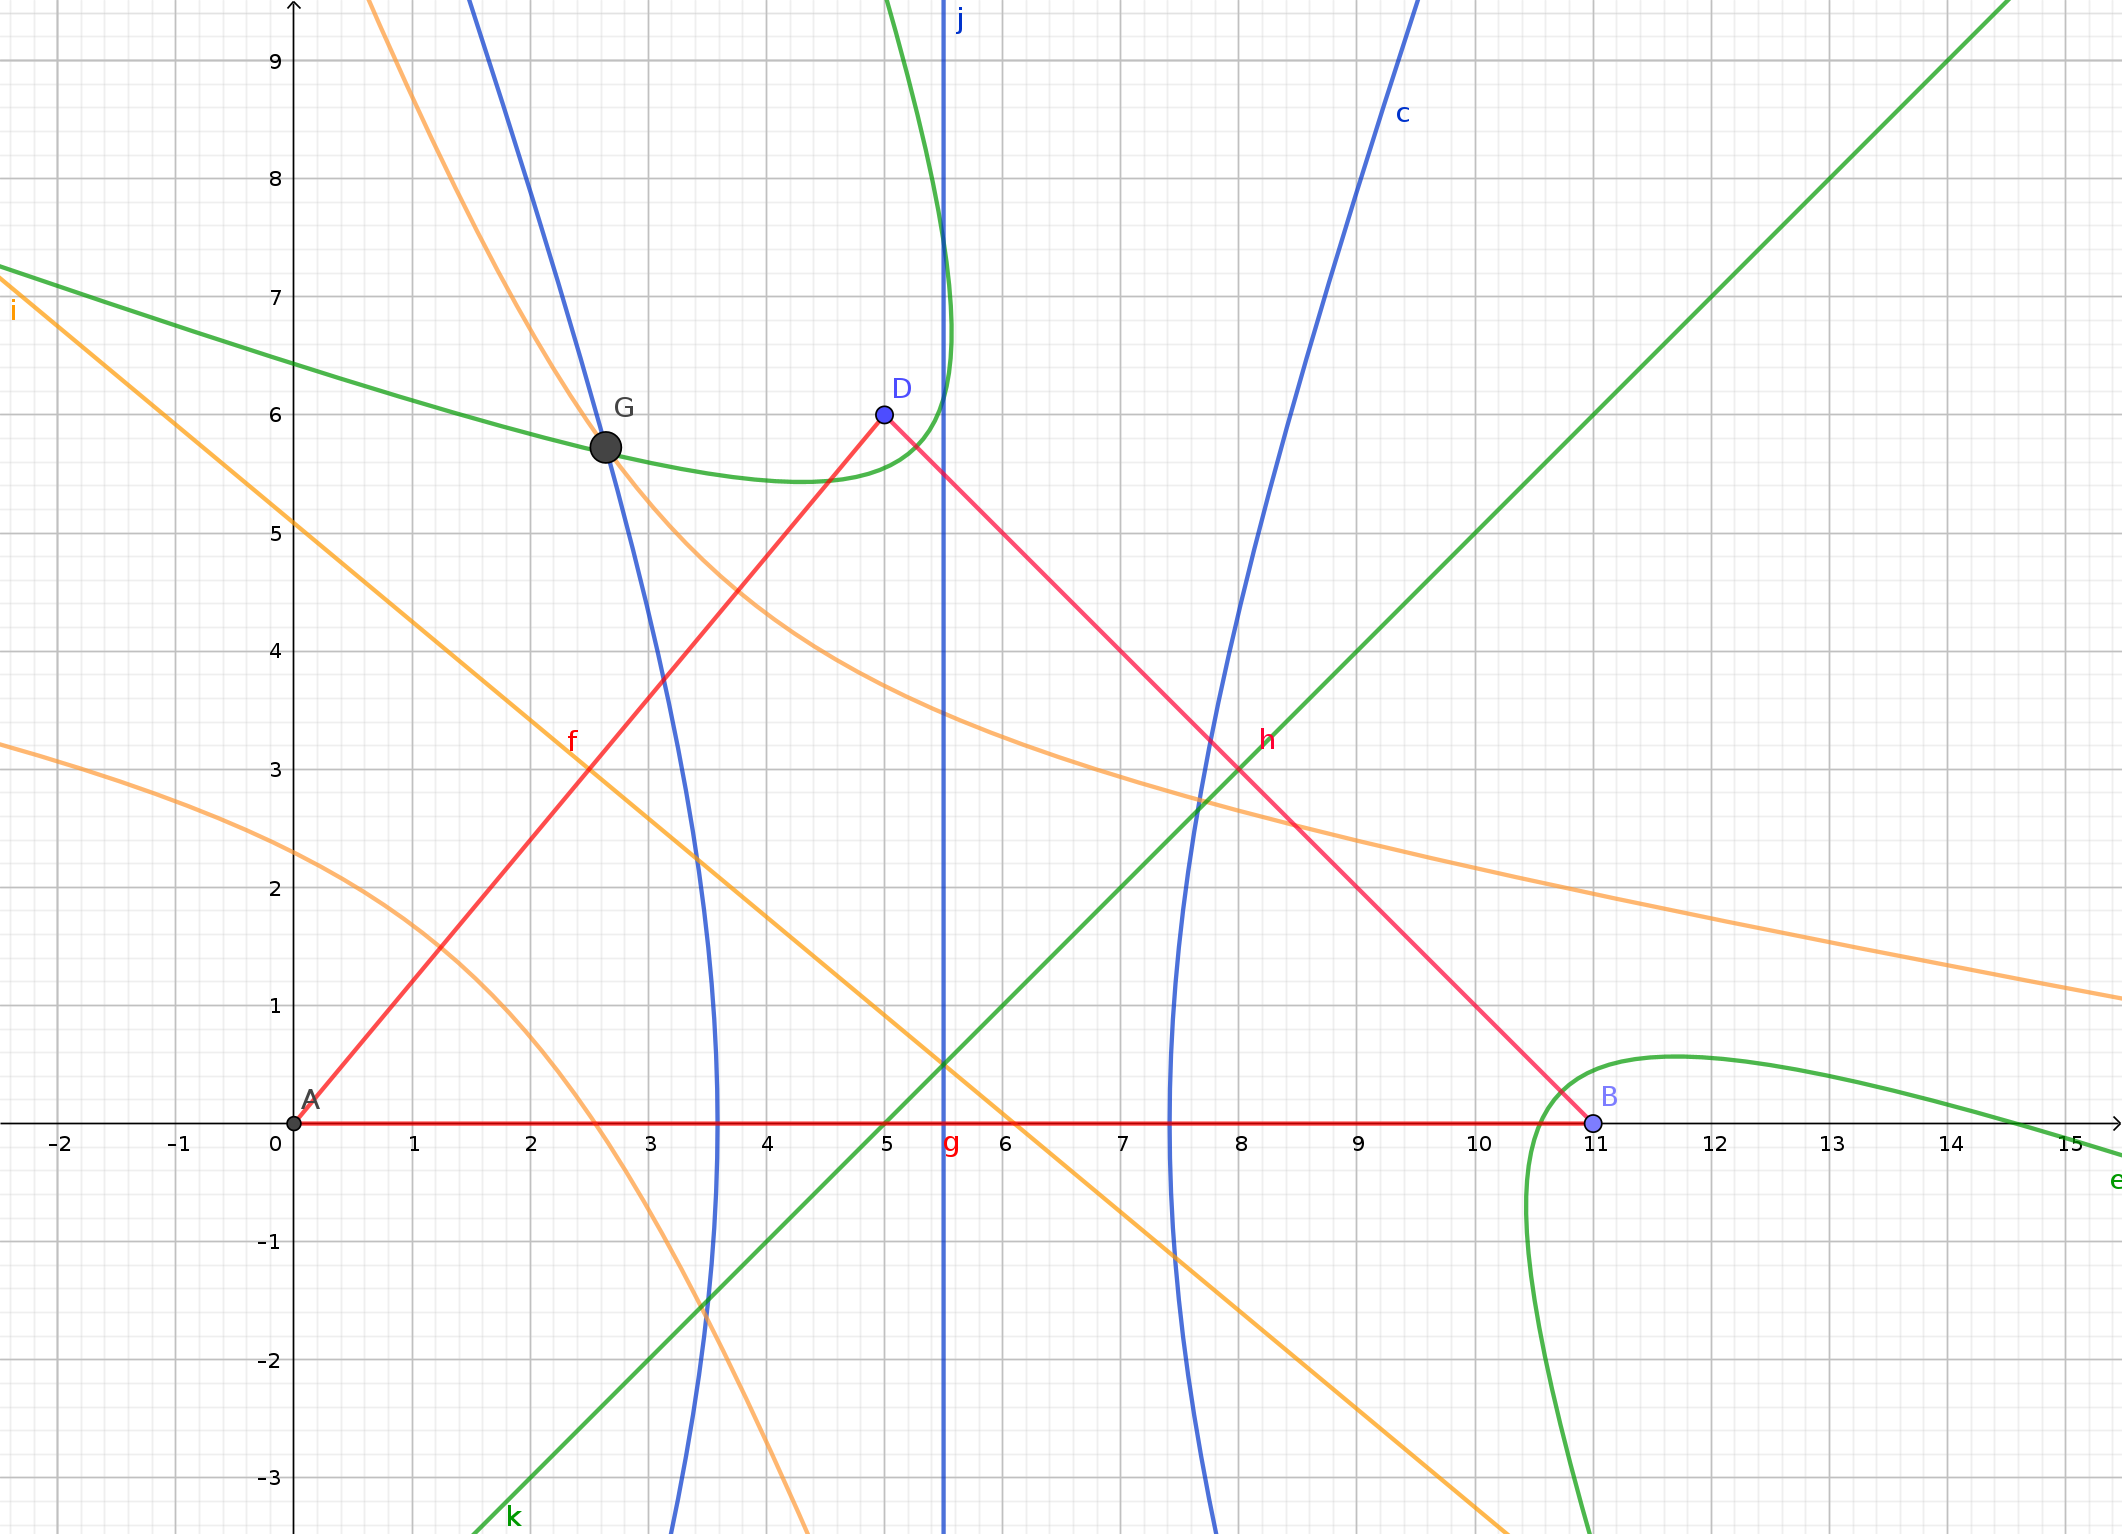
\includegraphics[width=0.9\textwidth]{tdoa.png}
    \caption{Time Difference of Arrival}
    \label{fig:tdoa}
\end{figure}

\subsection{Phase Difference of Arrival (PDoA)}
The PDoA method consists of combining the TWR scheme that delivers the distance between two devices with the measure of the bearing between the two devices. The combination of distance and bearing allows the calculation of the relative position of two devices without any other infrastructure. To do so, one of the devices carries two antennas and is able to measure the Phase Difference of Arrival of the RF signal.


Assume two antenna separated by a distance $d$, with a wavefront incident at an angle $\theta$, then the extra path the signal must travel between antenna 1 and antenna 2 (see figure \ref{fig:PhaseInterferometry}) results in a phase difference, \Delta\Phi, between the two antennas. This can be used to calculate the direction of arrival using:

\begin{equation}
    \theta = \arcsin(\frac{\lambda\Delta\Phi}{2\pi d})
\end{equation}

\begin{figure}[H]
    \centering
    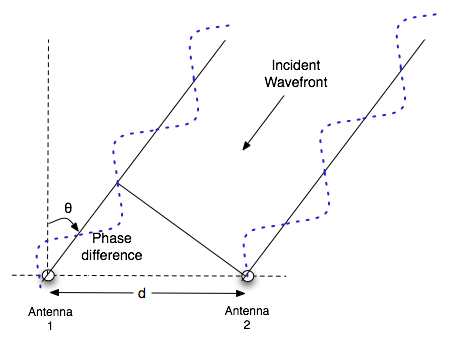
\includegraphics[width=0.7\textwidth]{PhaseInterferometry.png}
    \caption{Phase Difference of Arrival}
    \label{fig:PhaseInterferometry}
\end{figure}

\begin{figure}[H]
    \centering
    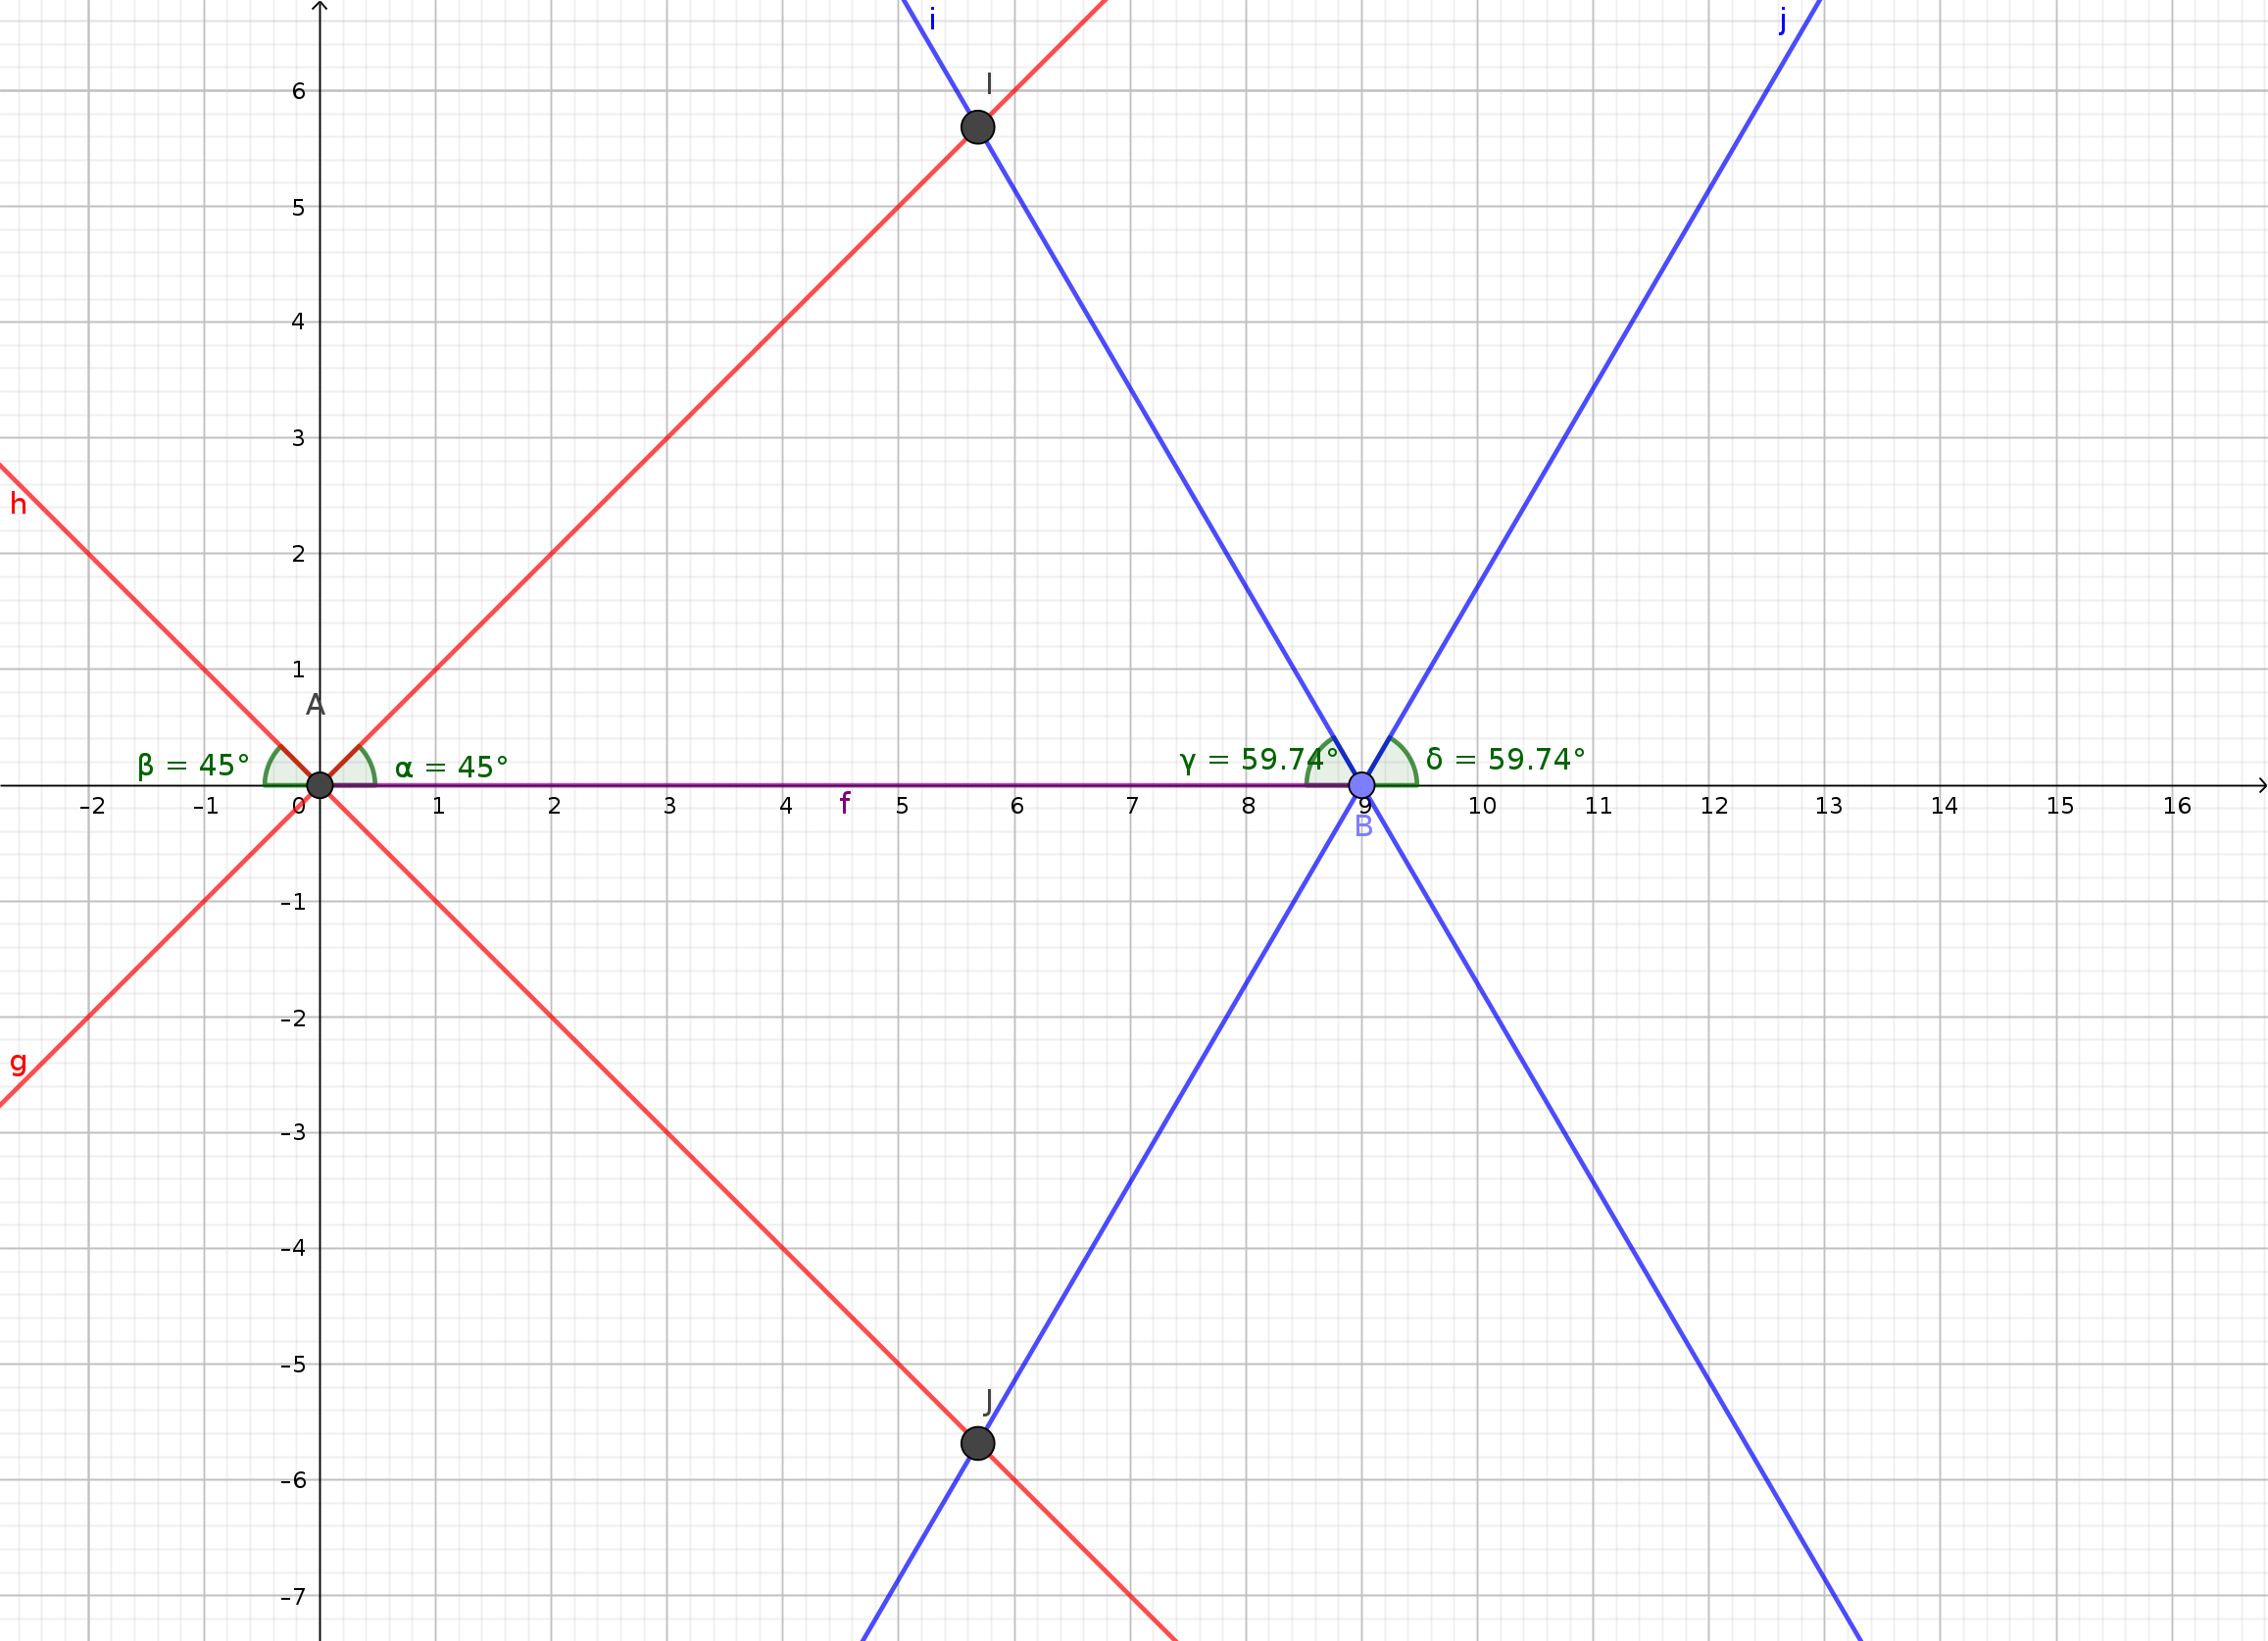
\includegraphics[width=0.9\textwidth]{pdoa.png}
    \caption{Phase Difference of Arrival}
    \label{fig:pdoa}
\end{figure}

\subsection{Two-Way Ranging (TWR)}
The TWR method relies on two-way communication between two devices. As they communicate, the devices also measure the Time of Flight of the UWB RF signal between them. By multiplying the round trip time of the signal by the speed of light, and then dividing by 2, you can derive the actual distance between the two devices. If you apply the TWR scheme between two devices, you will get the distance (D) between the two devices. Based on the TWR scheme, you can also implement 2D or even 3D location by measuring the distance between your mobile tags and fixed beacons – this is called triangulation.

\begin{figure}[H]
    \centering
    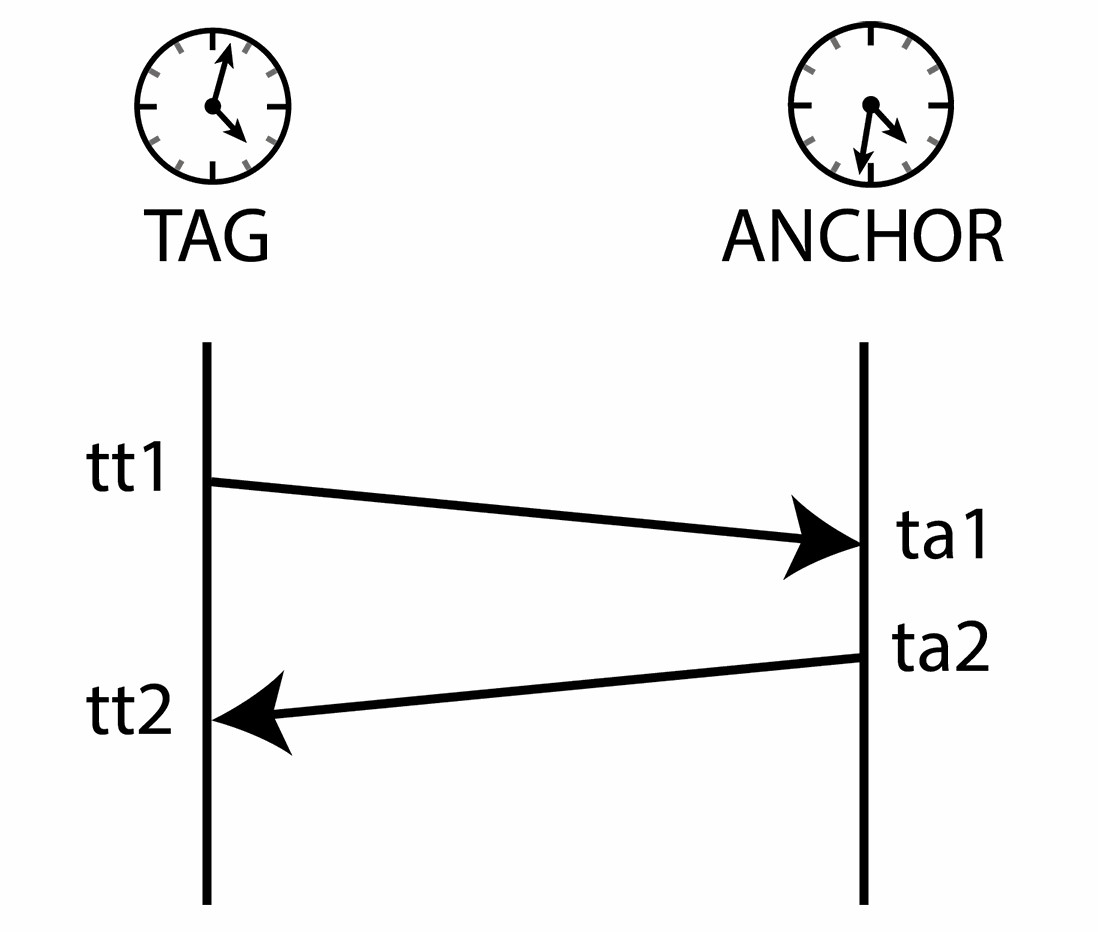
\includegraphics[width=0.3\textwidth]{twr_protocol.png}
    \caption{TWRImage}
    \label{fig:TWRImage}
\end{figure}

\begin{figure}[H]
    \centering
    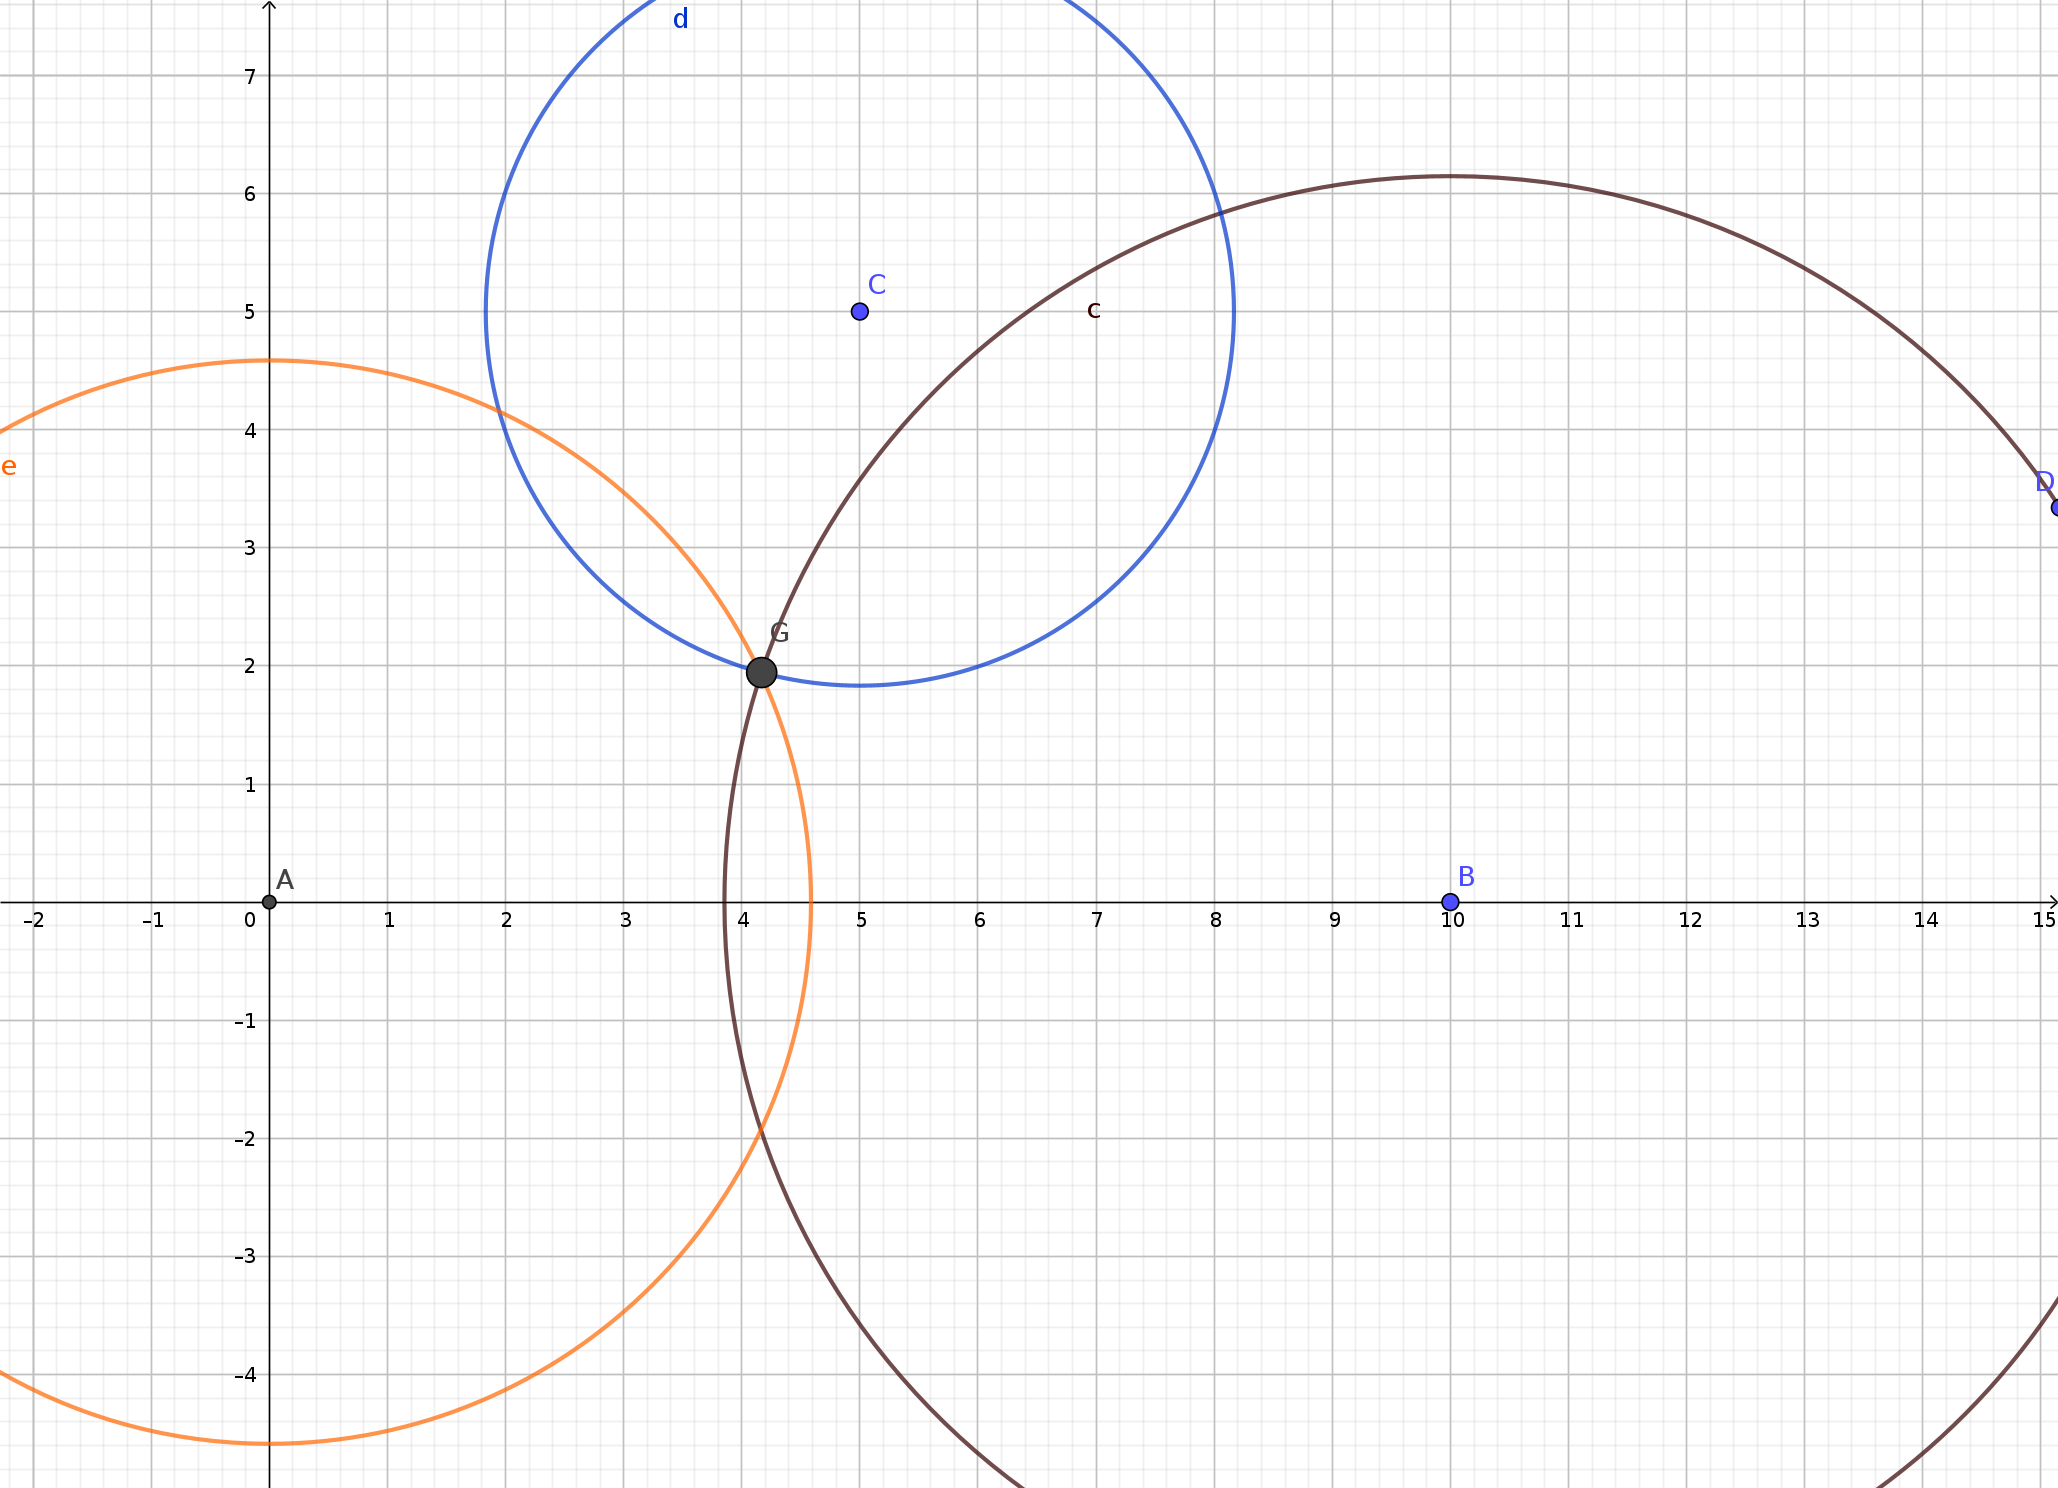
\includegraphics[width=0.9\textwidth]{twr.png}
    \caption{TWRImage}
    \label{fig:TWRImage}
\end{figure}

\section{Multilateration in three-dimensional Euclidean space}
\label{sec:localization_using_multilateration}

Suppose there are three unique anchor points in three dimensional space: $A_1(x_1, y_1,z_1)$, $A_2(x_2, y_2,z_2)$,
and $A_3(x_3, y_3,z_3)$ and an unknown tag point $T(x,y,z)$ with three known distances to each anchor point:
\begin{equation}
    \begin{split}
        d_1 = | T - A_1| \\
        d_2 = | T - A_2| \\
        d_3 = | T - A_3|
    \end{split}
\end{equation}
The problem of finding the coordinates of $T$ is called multilateration in 3D space. The name is derived from trilateration, a  geometrical problem of determining an unknown position on a plane based on the distance to other two known vertices of a triangle (the length of two sides). In this section, closed-form solution for multilateration problem is derived base on a simplified problem.

\subsection{Simplified problem}
\label{subsection:multilateration_simplified_problem}
For simplicity, assume that the three anchor points lie on the $xy$ plane with $z = 0$. Rewriting the coordinates of the three anchors: $A_1(0,0,0)$, $A_2(x_2,0,0)$, $A_3(x_3,y_3,0)$ with $x_2 \neq 0$, $x_3 \neq 0$ and $y_3 \neq 0$, then equation of the sphere associated with each anchor is as follows:
\begin{subequations}
    \begin{align}
        A_1 &\Rightarrow  x^2 + y^2 + z^2 = d_1^2 \label{eqn:d1_t_a_a}\\
        A_2 &\Rightarrow (x-x_2)^2 + y^2 + z^2 = d_2^2 \label{eqn:d1_t_a_b}\\
        A_3 &\Rightarrow (x-x_3)^2 + (y-y_3)^2 + z^2 = d_3^2 \label{eqn:d1_t_a_c}
    \end{align}
\end{subequations}
\begin{figure}[H]
    \centering
    \includegraphics[width=0.7\textwidth]{simplified_multilateration.png}
    \caption{Simplified multilateration}
    \label{fig:simplified_multilateration}
\end{figure}
Subtract equations \ref{eqn:d1_t_a_b} and \ref{eqn:d1_t_a_a} to solve for $x$:
\begin{equation}
    \begin{split}
        x_2^2 - 2x_2x + x^2 + y^2 + z^2 &= d_2^2\\
        x^2 + y^2 + z^2 &= d_1^2 \\
        \cline{1-2}
        x_2^2 - 2x_2x &= d_2^2 - d_1^2 \\
        \Leftrightarrow 2xx_2 &=  d_1^2 - d_2^2 + x_2^2 \\
        \Leftrightarrow x &= \frac{d_1^2 - d_2^2 + x_2^2}{2x_2}
    \end{split}
    \label{eqn:simplified_multilateration_x}
\end{equation}
Subtract equations \ref{eqn:d1_t_a_c} and \ref{eqn:d1_t_a_a} to solve for $y$:
\begin{equation}
    \begin{split}
        x_3^2  - 2x_3x + y_3^2 - 2y_3y + x^2 + y^2 + z^2 &= d_3^2 \\
        x^2 + y^2 + z^2 &= d_1^2 \\
        \cline{1-2}
        x_3^2  - 2x_3x + y_3^2 - 2y_3y &= d_3^2 - d_1^2\\
        \Leftrightarrow 2y_3y &= d_1^2 - d_3^2 + x_3^2 + y_3^2 - 2x_3x \\
        \Leftrightarrow y &= \frac{d_1^2 - d_3^2 + x_3^2 + y_3^2 - 2x_3x}{2y_3} \\
        &= \frac{d_1^2 - d_3^2 + x_3^2 + y_3^2 - \frac{x_3(d_1^2 - d_2^2 + x_2^2)}{x_2}}{2y_3}
    \end{split}
    \label{eqn:simplified_multilateration_y}
\end{equation}
Plug \ref{eqn:simplified_multilateration_x} and \ref{eqn:simplified_multilateration_y} into \ref{eqn:d1_t_a_a} for solving $z$:
\begin{equation}
    \begin{split}
        z &= \pm \sqrt{d_1^2 - x^2 - y^2} \\
        &= \pm \sqrt{d_1^2 - \left(\frac{d_1^2 - d_2^2 + x_2^2}{2x_2}\right)^2 - \left(\frac{d_1^2 - d_3^2 + x_3^2 + y_3^2 - \frac{x_3(d_1^2 - d_2^2 + x_2^2)}{x_2}}{2y_3}\right)^2}
    \end{split}
    \label{eqn:simplified_multilateration_z}
\end{equation}
There are unique solutions to the simplified multilateration problem, since the result of three intersecting spheres are two points.

\subsection{A closed-form solution for multilateration problem}
To fully solve the multilateration problem in Euclidean space, $A_1$, $A_2$, $A_3$ is firstly transformed to the coordinate as the above simplified problem. Since the distances are invariant under such transformation which are the linear and rotation transformation, $T$ can be found using \ref{eqn:simplified_multilateration_x}, \ref{eqn:simplified_multilateration_y} and \ref{eqn:simplified_multilateration_z}. $T$ is then transformed to the original coordinate to get the final result.

Let $S =\{\boldsymbol{e_x}, \boldsymbol{e_y}, \boldsymbol{e_z}\}$ is the basis of the new vector space. Then $A_1$, $A_2$, $A_3$ can be written uniquely as a linear combination of vectors in the basis $S$. Basis $S$ is specially chosen to make the general problem become the simplified problem. As shown in equation \ref{eqn:multilateration_ex}, $\boldsymbol{e_x}$ is a unit vector lies on $\overrightarrow{A_1A_2}$.
\begin{equation}
    \boldsymbol{e_x} = \frac{A_2-A_1}{\Vert A_2 - A_1\Vert}
    \label{eqn:multilateration_ex}
\end{equation}
Since $\Vert \boldsymbol{e_x} \Vert = 1$, the scalar projection of $\overrightarrow{A_1A_3}$ onto $\overrightarrow{A_1A_2}$ is:
\begin{equation}
    \begin{split}
    V_x &= \Vert A_3 - A_1 \Vert \cos{\gamma} \\
    &= \Vert \boldsymbol{e_x} \Vert \Vert A_3 - A_1 \Vert \cos{\gamma}\\
    &= \boldsymbol{e_x} \cdot (A_3 - A_1)      
    \end{split}
\end{equation}
The component of $\overrightarrow{A_1A_3}$ lies on $e_y$ is $A_3-A_1-(s*\boldsymbol{e_x})$. Hence:
\begin{equation}
    \boldsymbol{e_y} = \frac{A_3-A_1-(s*\boldsymbol{e_x})}{\Vert A_3-A_1-(s*\boldsymbol{e_x})\Vert}
\end{equation}
Finally, $\boldsymbol{e_z}$ is the cross product of the two other unit vectors.
\begin{equation}
    \boldsymbol{e_z} = \boldsymbol{e_x} \times \boldsymbol{e_y}
\end{equation}
\begin{figure}[H]
    \centering
    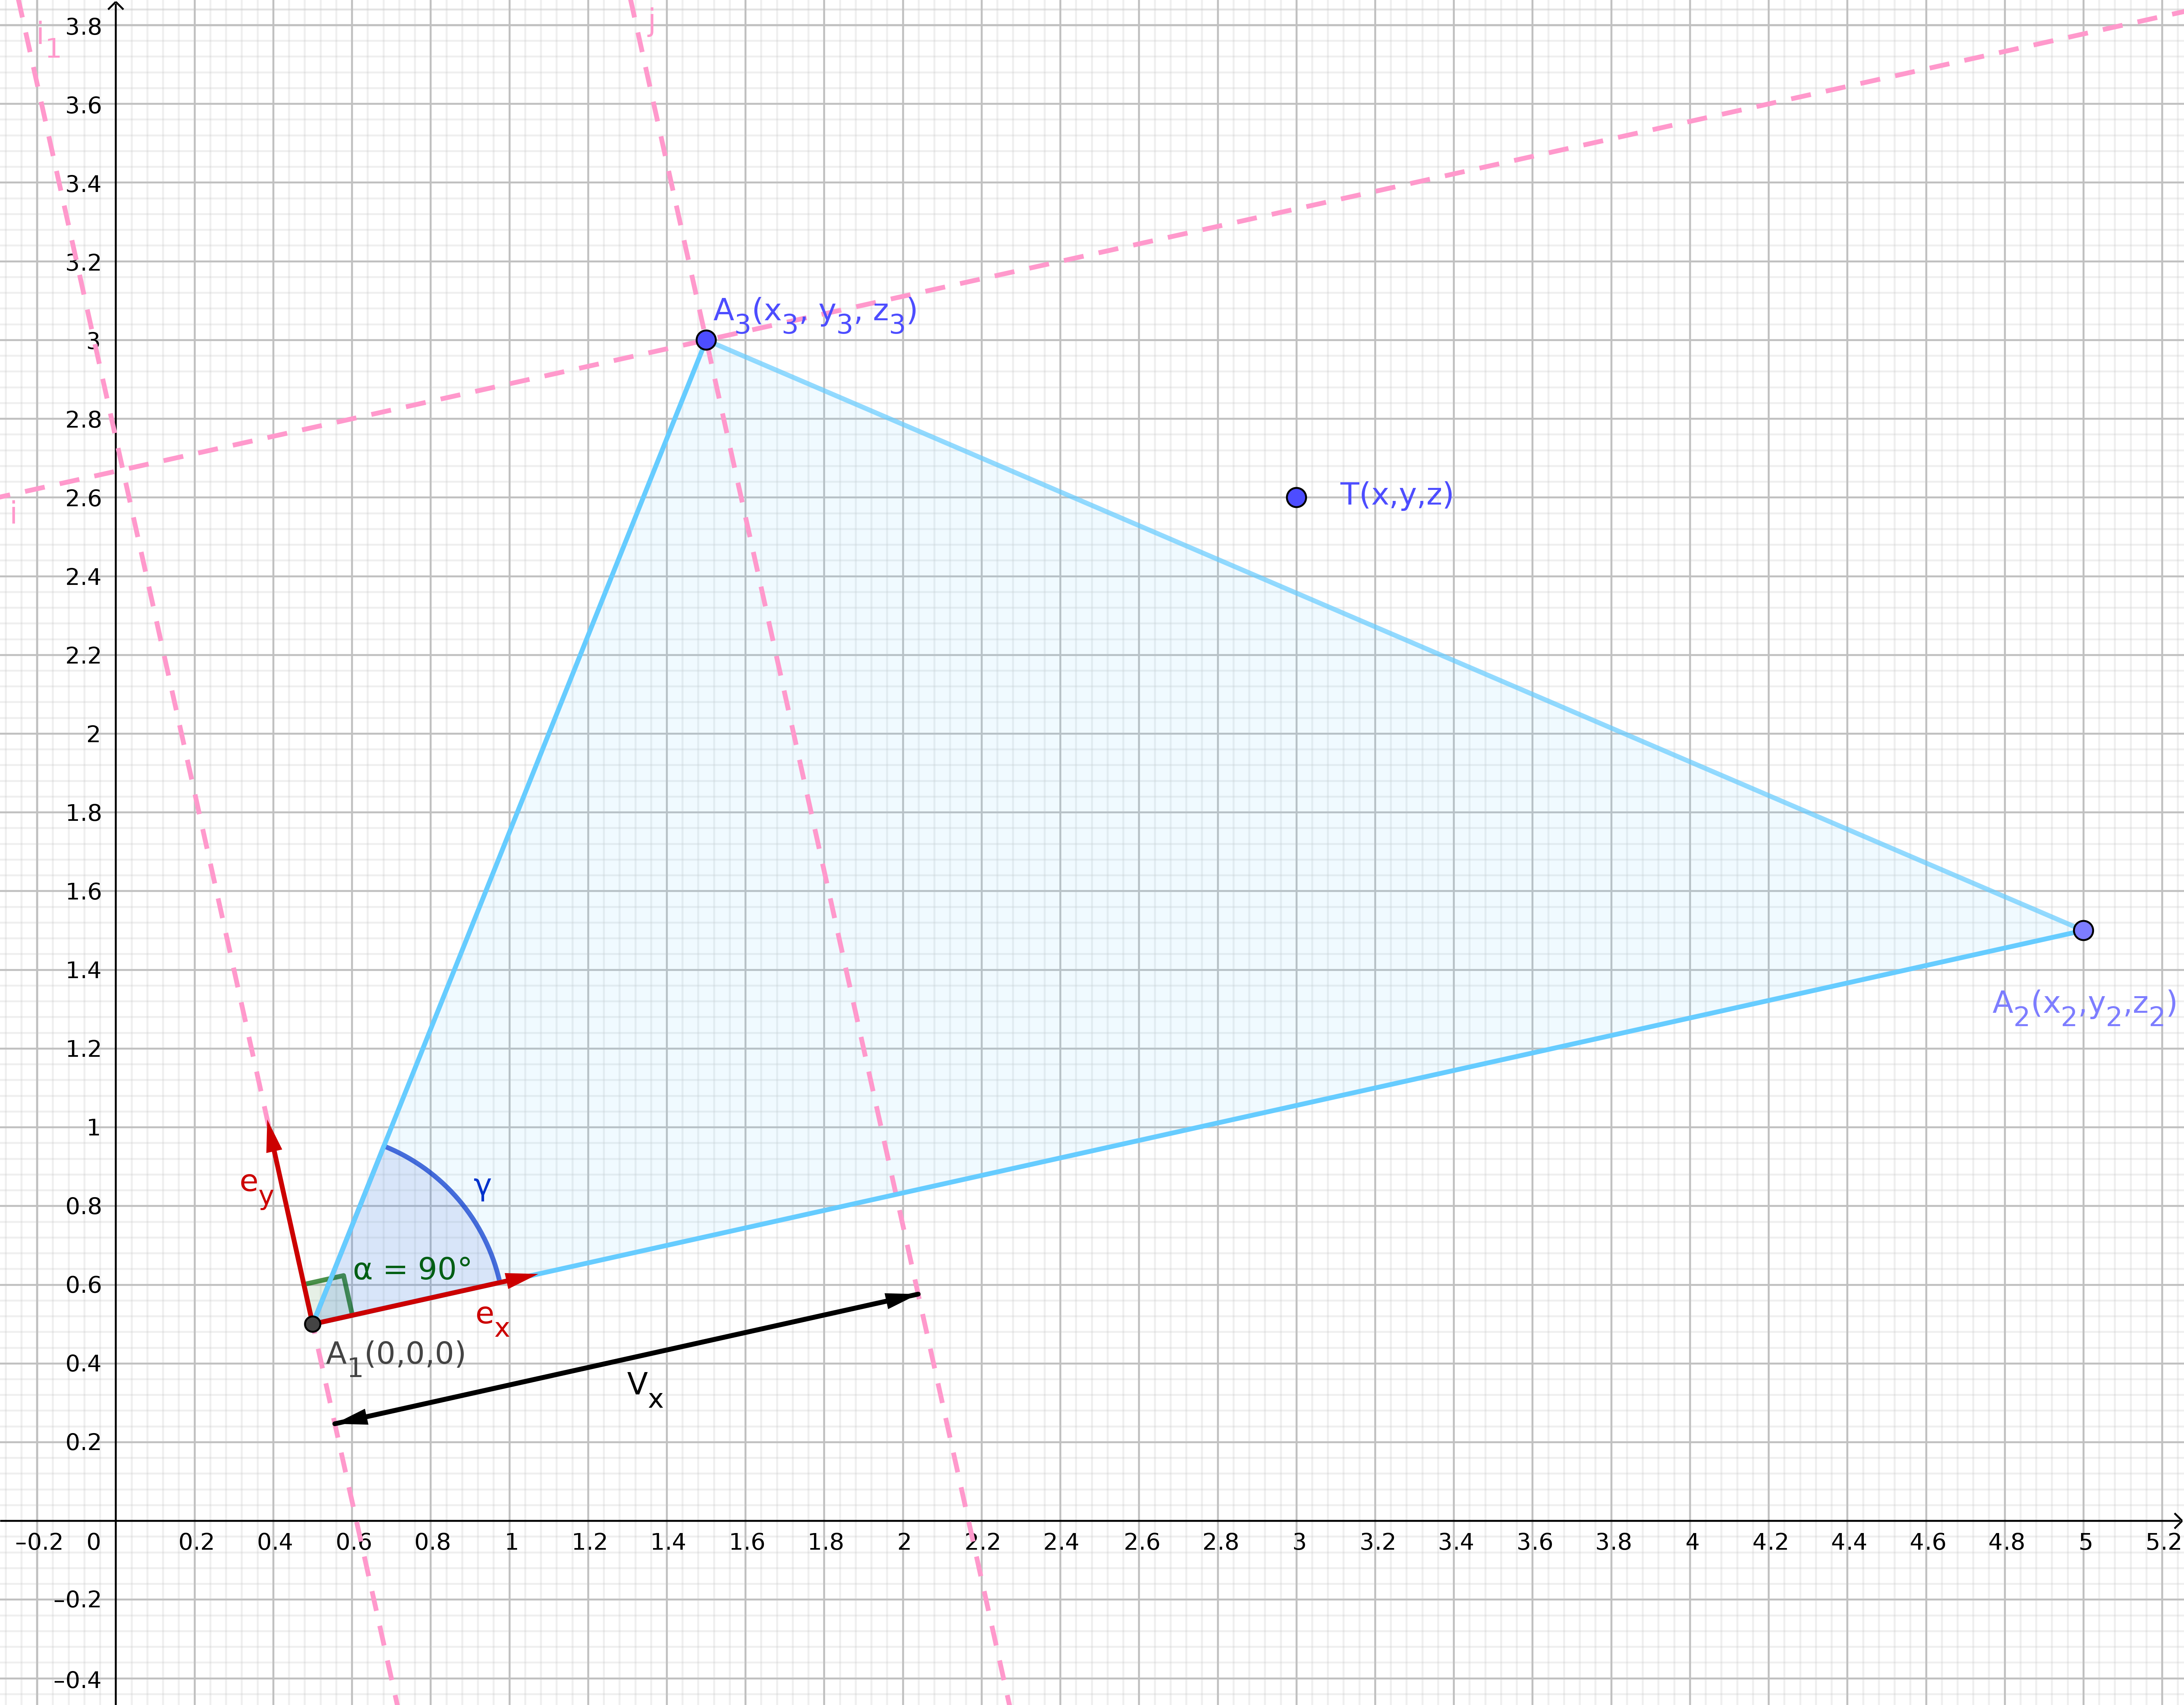
\includegraphics[width=0.7\textwidth]{multilateration.png}
    \caption{Multilateration in Euclidean space}
    \label{fig:multilateration}
\end{figure}

In the basis $S$, the new set of points is:
\begin{equation}
    \begin{split}
        &B_0(0,0,0) \\
        &B_1(U, 0, 0) = B_1(\Vert A_2 - A_1 \Vert, 0, 0) \\
        &B_2(V_x, V_y, 0) = B_2(\boldsymbol{e_x} \cdot (A_3 - A_1), \boldsymbol{e_y} \cdot (A_3 - A_1), 0) 
    \end{split}
    \label{eqn:multilateration_to_simplified_problem}
\end{equation}
As the distance is invariant to basis change, the coordinates of $T$ in the $S$ basis can be found using \ref{eqn:multilateration_to_simplified_problem} as described in section \ref{subsection:multilateration_simplified_problem}.

Suppose that the coordinates of $T$ found in the basis $S$ are $T'_1(x_t,y_t,z_t)$ and $T'_2(x_t, y_t, -z_t)$, the coordinates of $T$ in the original coordinate can calculated using equation \ref{eqn:multilateration_inverse_transfrom}.
\begin{equation}
    \begin{split}
        T_1 = A_1 + x_t\boldsymbol{e_x} + y_t\boldsymbol{e_y} + z_t\boldsymbol{e_z} \\
        T_2 = A_1 + x_t\boldsymbol{e_x} + y_t\boldsymbol{e_y} - z_t\boldsymbol{e_z} 
    \end{split}
    \label{eqn:multilateration_inverse_transfrom}
\end{equation}

\subsection{Multilateration implementation}
A python implementation for multilateration in Euclidean space is shown in figure \ref{fig:multilateration_python_implementation}.
\begin{figure}[H]
    \begin{python}
import numpy as np

def multilateration(distances):
    A1=np.array(distances[0][:3])
    A2=np.array(distances[1][:3])
    A3=np.array(distances[2][:3])
    d1=distances[0][-1]
    d2=distances[1][-1]
    d3=distances[2][-1]

    U=np.linalg.norm(A2-A1)
    e_x=(A2-A1)/U
    Vx=np.dot(e_x,(A3-A1))
    e_y=(A3-A1-(Vx*e_x))/(np.linalg.norm(A3-A1-(Vx*e_x)))
    Vy=np.dot(e_y,(A3-A1))
    e_z=np.cross(e_x,e_y)

    x=(d1**2-d2**2+U**2)/(2*U)
    y=(d1**2-d3**2+Vx**2+Vy**2-2*Vx*x)/(2*Vy)
    z1=np.sqrt(d1**2-x**2-y**2)
    z2=-z1

    T1=A1+(x*e_x)+(y*e_y)+(z1*e_z)
    T2=A1+(x*e_x)+(y*e_y)+(z2*e_z)
    return T1, T2
    \end{python}
    \caption{Python code for multilateration in Euclidean space}
    \label{fig:multilateration_python_implementation}
\end{figure}

On a real scenario, distances to other known points are used for selecting the final location from the two locations. The chosen location should have a distance to the known point being closest to the given one. If multiple distances are available, voting may be one solution.
\end{document}